\documentclass{article}

% Bibliography
\usepackage{natbib}
\bibpunct{(}{)}{;}{a}{}{;}

% Use 'It was found that A is B (Name 1234)' style
\setcitestyle{authoryear,open={},close={}}

% Affiliations
\usepackage{authblk}
\title{pirouette: the error BEAST2 makes in inferring a phylogeny}
\author[1]{Rich\`el J.C. Bilderbeek}
\author[1]{Giovanni Laudanno}
\author[1]{Rampal S. Etienne}
\affil[1]{Groningen Institute for Evolutionary Life Sciences, University of Groningen, Groningen, The Netherlands}

% Use double spacing
\usepackage{setspace}
\doublespacing

\usepackage{listings}
\usepackage{hyperref}
\usepackage{todonotes}
\usepackage{verbatim}
\usepackage{pgf}
\usepackage{bm}

% sidewaysfigure
\usepackage{rotating}

% Style of listings
% From http://r.789695.n4.nabble.com/How-to-nicely-display-R-code-with-the-LaTeX-package-listings-tp4648110.html
\usepackage{fancyvrb} 
\definecolor{codegreen}{rgb}{0,0.6,0}
\definecolor{codegray}{rgb}{0.5,0.5,0.5}
\definecolor{codepurple}{rgb}{0.58,0,0.82}
\definecolor{backcolor}{rgb}{0.95,0.95,0.92}
\lstdefinestyle{mystyle}{
  language=R,% set programming language
  basicstyle=\ttfamily\small,% basic font style
  commentstyle=\color{gray},% comment style
  % numbers=left,% display line numbers on the left side
  numberstyle=\scriptsize,% use small line numbers
  numbersep=10pt,% space between line numbers and code
  tabsize=2,% sizes of tabs
  showstringspaces=false,% do not replace spaces in strings by a certain character
  captionpos=b,% positioning of the caption below
  breaklines=true,% automatic line breaking
  escapeinside={(*}{*)},% escaping to LaTeX
  fancyvrb=true,% verbatim code is typset by listings
  extendedchars=false,% prohibit extended chars (chars of codes 128--255)
  alsoletter={.<-},% becomes a letter
  alsoother={$},% becomes other
  otherkeywords={!=, ~, $, \&, \%/\%, \%*\%, \%\%, <-, <<-, /},% other keywords
  deletekeywords={c}% remove keywords 
}
\lstset{style=mystyle}

% Adds numbered lines
\usepackage{lineno}
\linenumbers

% Rename 'Abstract' to 'Summary 
\usepackage[english]{babel}
\addto{\captionsenglish}{\renewcommand{\abstractname}{Summary}}

%comments
\newcommand{\giovanni}[1]{\textcolor{blue}{\textbf{[GL: #1]}}}
\newcommand{\richel}[1]{\textcolor{orange}{\textbf{[RB: #1]}}}

\begin{document}

\maketitle

\begin{abstract}

  \textbf{1. }
    BEAST2 is a popular Bayesian phylogenetics software tool,
    that takes an alignment and inference model to create a
    posterior of jointly-estimated phylogenies and model parameter estimates.
    When a new macro-evolutionary diversification model is developed,
    a good first step is to measure the error BEAST2 makes on a known
    phylogeny derived from a new diversification mechanism, 
    with its current set of inference models. \\
  \textbf{2. }
    Here, we present a free, libre and open-source R package, \verb;pirouette;
    that assesses the inference error BEAST2 makes based on a known/true 
    phylogeny. \\
  \textbf{3. }
    We describe \verb;pirouette;'s usage and the biological scientific
    question it can answer, including full examples. \\
  \textbf{4. }
    As \verb;pirouette; is designed to be of high quality and extendable, 
    we conclude by describing the further development of the package. \\
\end{abstract}

{\bf Keywords:} computational biology, evolution, phylogenetics, BEAST2, pirouette, R





%%%%%%%%%%%%%%%%%%%%%%%%%%%%%%%%%%%%%%%%%%%%%%%%%%%%%%%%%%%%%%%%%%%%%%%%%%%%%%%%%%%%%%
\section{Introduction}
%%%%%%%%%%%%%%%%%%%%%%%%%%%%%%%%%%%%%%%%%%%%%%%%%%%%%%%%%%%%%%%%%%%%%%%%%%%%%%%%%%%%%%


Phylogenies are commonly used to explore evolutionary hypotheses.
The mode of diversification is one such hypothesis.
Phylogenies constructed from DNA alignments are commonly fit to
diversification models, or the other way around. For example,
[Etienne $\&$ Rosindell 2012] fit four bird phylogenies to the protracted
diversification model.
\giovanni{ALTERNATIVE VERSION: The development of new powerful inference tools, such as BEAST [\cite{drummond2007beast}] or MrBayes [\cite{huelsenbeck2001mrbayes}], provided us the possibility to build phylogenetic trees from genetic material extracted from extant organisms. This has constituted a big step forward in the general understanding on how species evolved (this can be improved). Having access to this new kind of data has given rise to a high interest in understanding what are the main drivers and modes for diversification processes. }

There are plenty of diversification models: constant-birth [Yule, 19..],
birth-death [\cite{nee1994reconstructed}], time-dependent [?], diversity 
dependent [\cite{etienne2011diversity}], protracted 
birth-death [\cite{rosindell2010protracted}][\cite{etienne2012prolonging}],
multiple-birth death [Laudanno, Bilderbeek, Haegeman $\&$ Etienne, in preparation],
a rate shifting birth-death model [the SLS model. Laudanno, Haegeman $\&$ Etienne, in preparation]
punctuated equilibrium aka early burst [?Harmon],
dependent on a binary trait [\cite{maddison2007estimating}], 
multiple state trait [\cite{fitzjohn2012diversitree}],
concealed state [\cite{beaulieu2016detecting}] or even a combination of multiple concealed and observable states [\cite{herrera2018detecting}].
\giovanni{
@Richel: I am wondering if it might be worth to give a brief explanation on the philosophy of the aforementioned models, to explain why we want to simulate the processes. In case, this could be a stub for it:
Such models usually rely on the assumption that a particular diversification process can be explained mainly by specific mechanisms.
Such mechanisms are built into likelihood functions, which provide the likelihood of the parameters, given the data.
By maximizing the likelihood is possible to give the best inference of such parameters. It is therefore a standard practice, to validate such models, to test them versus simulated processes generated according to the hypothesised mechanisms.
}
Diversification models are getting more complex over time. There are many
reasons for this. One reason is the increase in computing power,
which allows this heightened complexity possible.
Another reason is to explore a process that is not
yet captured by the other diversification models. An example of this
is the multiple-birth model [Laudanno, Bilderbeek, Haegeman $\&$ Etienne, in preparation], 
that is the first model to allow speciation to co-occur.

An open question for each new diversification model is whether the increased
complexity is worth the extra computational resources \giovanni{I think here it is not only a matter of computational resources. I believe there two more factors: 1) developing a likelihood model takes time, human resources and therefore fundings; 2) in principle you can elaborate any model to be as complex as possibly requested, however there is a diminishing return on this. In fact the purpose of modelling for complex systems such as biology is to hypothesize the main driving factors of a process and trying to prove that they are indeed able to explain the main features of the phenomenon you want to explain. In my opinion the job of a modeller is to try to disentangle the intrinsic complexity of a system highlighting the main reasons of its behaviour. In such a light you don't want your model to be unnecessary complex.}. There are many
ways to answer this question. One possible experiment 
is to use a phylogeny of the new diversification model,
simulate its alignment and see how well our
current inference models are at retrieving the phylogeny.
If this difference is small enough, current models apparently
suffice.

\verb;pirouette; is an R package that performs such an experiment,
and is built on \verb;babette; [Bilderbeek $\&$ Etienne, 2018], 
which calls the popular Bayesian inference tool 
BEAST2 [\cite{bouckaert2014beast}]. With \verb;pirouette;, one
can easily measure the error made by Bayesian inference in recovering
any given phylogeny, helping us to valorize new diversification models.

%%%%%%%%%%%%%%%%%%%%%%%%%%%%%%%%%%%%%%%%%%%%%%%%%%%%%%%%%%%%%%%%%%%%%%%%%%%%%%%%%%%%%%
\section{Description}
%%%%%%%%%%%%%%%%%%%%%%%%%%%%%%%%%%%%%%%%%%%%%%%%%%%%%%%%%%%%%%%%%%%%%%%%%%%%%%%%%%%%%%

\verb;pirouette; is written in the R programming language (\cite{R}).

\begin{sidewaysfigure}
  \centering
  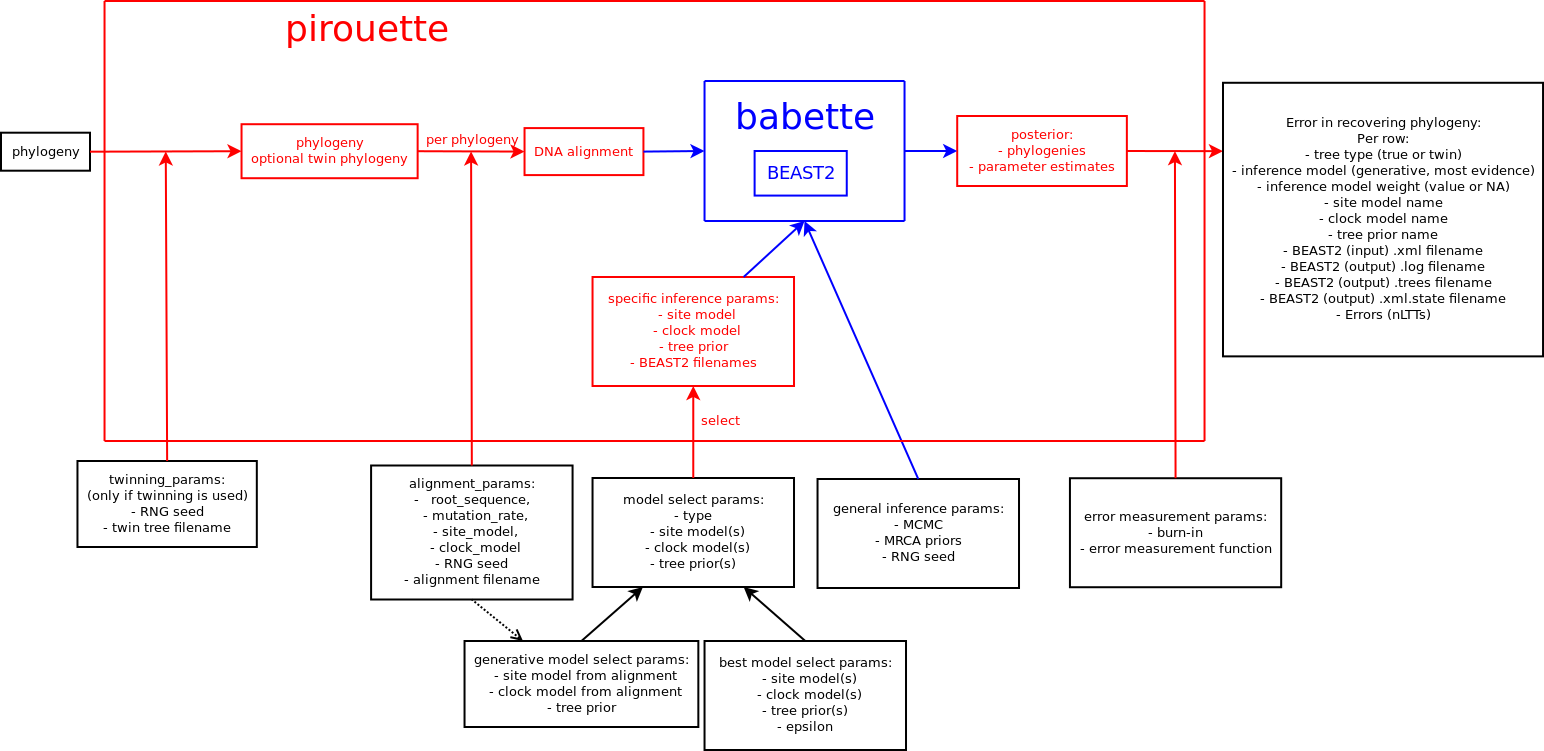
\includegraphics[width=\textwidth]{overview.png}
  \caption{pirouette pipeline}
  \label{fig:pipeline}
\end{sidewaysfigure}

The goal of \verb;pirouette; is to measure the inference error BEAST2
makes from a given phylogeny of which full information is provided \giovanni{is this true? do we also provide information about extinct species or we just use reconstructed tree (which always lack a lot of information)?}.

The pipeline is summarized by the following steps, which will be described in detail below:
\begin{enumerate}
    \item from a given phylogeny an alignment is simulated;
    \item from the alignment an inference model is chosen;
    \item the alignment is used as BEAST2 input to infer a posterior distribution of phylogenies;
    \item posterior phylogenies are compared with the given phylogenies to estimate the error we make. The bigger the match, the lower the error;
\end{enumerate}
There is also the option to generate a 'twin tree',
that goes through the same pipeline.

The first step simulates a DNA alignment from the given phylogeny.
One can specify a DNA sequence
of any length at the root of the phylogeny, a DNA mutation rate, a
site (i.e. nucleotide substitution) model, 
a clock model, a random number generator (RNG) seed and a location
where the alignment is saved to. This step is relatively fast, but longer
DNA alignments will noticeably slow down the inference step.

The second step selects an inference model, using the alignment.
The user can specify whether to use the generative model or select a best model
from a set of inference models. 
When selecting the generative model,
the site and clock model used in the alignment simulation are used
in the inference. Because the given phylogeny (on which the alignment is based)
may have followed any tree prior (i.e. speciation model), the user needs
to specify which tree prior is used in the inference. 
When selecting for the best
model, the alignment is used to find the inference model that has the
highest evidence (i.e. marginal likelihood) from a set of inference models.
The evidence of an inference model is estimated using a nested sampling (NS)
approach, as described in \cite{maturana2018model}. The nested sampling is
performed by \verb;babette;, that call the 'NS' BEAST2 package. 
Using BEAST2 packages (in a scripted way) can only be done under Linux and Mac; 
inference model selection is not available on Windows.

The third step infers a Bayesian posterior from the simulated alignment,
using the inference model(s) selected in the previous step. The user
can specify the additional parameters needed for the BEAST2 run, which
are the Markov-Chain Monte Carlo (MCMC) setup, 
an optional Most Recent Common Ancestor (MRCA) prior and an RNG seed.
The MCMC setup determines the number of posterior trees sampled.
An MRCA prior allows the inferred phylogeny to have a dated crown age.

The fourth step measures the inference error, using the phylogenies in the
Bayesian posterior. These phylogenies are compared to the given
phylogeny using an error statistic, which is the nLTT 
statistic (\cite{janzen2015approximate}) by default,
but also a custom error statistic is supplied, based
on the absolute difference in the gamma statistic [Pybus $\&$ Harvy]. 
Additionally, the user can specify the
proportion of posterior phylogenies to 
discard (i.e. the burn-in), throwing away the first $10\%$
of all phylogenies by default. This burn-in is used to discard
the part of the MCMC chain that has not yet converged to a
representative part of state space.

An optional step is to generate a 'twin tree', that will be
analyzed in the same way as the true tree. The twin tree has the same
topology as the given phylogeny, yet its branch lengths follow the same
distribution as a Yule (pure-birth) or (constant rate) birth-death tree prior.
The use of such a twin tree, is to assess the minimum level of noise (i.e. 
error) BEAST2 makes when the input (the twin phylogeny) has an ideal branch
length distribution.

%%%%%%%%%%%%%%%%%%%%%%%%%%%%%%%%%%%%%%%%%%%%%%%%%%%%%%%%%%%%%%%%%%%%%%%%%%%%%%%%%%%%%%
\section{Installation}
%%%%%%%%%%%%%%%%%%%%%%%%%%%%%%%%%%%%%%%%%%%%%%%%%%%%%%%%%%%%%%%%%%%%%%%%%%%%%%%%%%%%%%

\verb;pirouette; can be installed easily from CRAN:

\begin{lstlisting}[language=R, floatplacement=H]
install.packages("pirouette")
\end{lstlisting}

For the most up-to-date version, 
one can download and install the package from \verb;pirouette;'s GitHub repository:

\begin{lstlisting}[language=R, floatplacement=H]
usethis::install_github("richelbilderbeek/pirouette")
\end{lstlisting}

To start using \verb;pirouette;, load its functions in the global namespace first:

\begin{lstlisting}[language=R, floatplacement=H]
library(pirouette)
\end{lstlisting}
Because \verb;pirouette; calls BEAST2, BEAST2 must be installed. 
This can be done from within R, using:

\begin{lstlisting}[language=R, floatplacement=H]
install_beast2()
\end{lstlisting}
For the option to select inference models,
\verb;pirouette; uses the "NS" BEAST2 package [Maturana et al.].
It can be installed from within R, using:

\begin{lstlisting}[language=R, floatplacement=H]
install_beast2_pkg("NS")
\end{lstlisting}

%%%%%%%%%%%%%%%%%%%%%%%%%%%%%%%%%%%%%%%%%%%%%%%%%%%%%%%%%%%%%%%%%%%%%%%%%%%%%%%%%%%%%%
\section{Usage: first research question}
%%%%%%%%%%%%%%%%%%%%%%%%%%%%%%%%%%%%%%%%%%%%%%%%%%%%%%%%%%%%%%%%%%%%%%%%%%%%%%%%%%%%%%

A first research question that \verb;pirouette; answers is:
What is the error BEAST2 makes from a phylogeny using the same 
diversification model as it was generated by?

We start with an idealised birth-death tree of five taxa and a crown age of 10:

% Need idealised birth-death tree
% From https://github.com/richelbilderbeek/pirouette_article/issues/1
% and https://github.com/richelbilderbeek/pirouette/issues/35
\begin{lstlisting}[language=R, floatplacement=H]
phylogeny <- ape::read.tree(text = "((A:4, B:4):1, (C:4, D:4):1);")
\end{lstlisting}

The first step in \verb;pirouette; is to simulate a DNA alignment from the 
given phylogeny. To do so, we must specify the DNA root sequence
and a mutation rate. In this example, the DNA root sequence consists
out of four block of 250 nucleotides each, where the per-nucleotide
mutation rate is 0.1 mutations per unit time.

\begin{lstlisting}[language=R, floatplacement=H]
alignment_params <- create_alignment_params(
  root_sequence = create_blocked_dna(length = 1000),
  mutation_rate = 0.1
)
\end{lstlisting}

The second step is to select how an inference model is picked.
We just select the generative model, which consists in a collection of 
three elements: a site model \giovanni{do we have to explain what a site model is or what are the options?}, a clock
model of the alignment and a birth-death tree prior
to be the generative tree prior. \giovanni{would it be helpful to the reader to explicit that site and clock models are automatically taken from the generative model?}

\begin{lstlisting}[language=R, floatplacement=H]
model_select_param <- create_gen_model_select_param(
  alignment_params = alignment_params,
  tree_prior = create_bd_tree_prior()
)
\end{lstlisting}

The third and fourth step have sensible defaults, and we are not
interested in using a twin tree. We can now measure the errors BEAST2
makes when inferring the given phylogeny in this way:

\begin{lstlisting}[language=R, floatplacement=H]
errors <- pir_run(
  phylogeny,
  alignment_params = alignment_params,
  model_select_params = model_select_param
)
\end{lstlisting}

\verb;pirouette; has a nice plotting function:

\begin{lstlisting}[language=R, floatplacement=H]
pir_plot(errors)
\end{lstlisting}

% TODO: write script to create figure 2, see
% https://github.com/richelbilderbeek/pirouette/issues/37
The resulting figure is shown in figure 2.

%%%%%%%%%%%%%%%%%%%%%%%%%%%%%%%%%%%%%%%%%%%%%%%%%%%%%%%%%%%%%%%%%%%%%%%%%%%%%%%%%%%%%%
\section{Usage: second research question}
%%%%%%%%%%%%%%%%%%%%%%%%%%%%%%%%%%%%%%%%%%%%%%%%%%%%%%%%%%%%%%%%%%%%%%%%%%%%%%%%%%%%%%

A second research question that \verb;pirouette; answers, is:
What is the error BEAST2 makes from a phylogeny when
picking the best inference model?

Here we start with a tree generated from an unknown 
diversification model, that has four taxa and a crown age of 5:

% Need idealised birth-death tree
% From https://github.com/richelbilderbeek/pirouette_article/issues/1
% and https://github.com/richelbilderbeek/pirouette/issues/35
\begin{lstlisting}[language=R, floatplacement=H]
phylogeny <- ape::read.tree(text = "((A:4, B:4):1, (C:4, D:4):1);")
\end{lstlisting}

The first step in \verb;pirouette; is to simulate a DNA alignment from the 
given phylogeny. We'll re-use the alignment parameters of the previous example \giovanni{it might be nice to add an explicit ref to the alignmentparams code}.

The second step is to select how an inference model is picked.
We will let the inference model that has the highest evidence be used
in the Bayesian inference. By default, \verb;pirouette; will try
all combinations of site models, clock models and tree priors.

\begin{lstlisting}[language=R, floatplacement=H]
model_select_param <- create_best_model_select_param()
\end{lstlisting}

Also here, the third and fourth step have sensible defaults, and we are not
interested in using a twin tree. We can now measure the errors BEAST2
makes when inferring the given phylogeny like this:

\begin{lstlisting}[language=R, floatplacement=H]
errors <- pir_run(
  phylogeny,
  alignment_params = alignment_params,
  model_select_params = model_select_param
)
\end{lstlisting}

Again, showing the results:

\begin{lstlisting}[language=R, floatplacement=H]
pir_plot(errors)
\end{lstlisting}

% TODO: write script to create figure 3, see
% https://github.com/richelbilderbeek/pirouette/issues/38
The resulting figure is shown in figure 3.

%%%%%%%%%%%%%%%%%%%%%%%%%%%%%%%%%%%%%%%%%%%%%%%%%%%%%%%%%%%%%%%%%%%%%%%%%%%%%%%%%%%%%%
\section{Usage: third research question}
%%%%%%%%%%%%%%%%%%%%%%%%%%%%%%%%%%%%%%%%%%%%%%%%%%%%%%%%%%%%%%%%%%%%%%%%%%%%%%%%%%%%%%

A third research question that \verb;pirouette; answers is:
What is the error BEAST2 makes from a phylogeny 
picking the best inference model, compared to the background noise?

We use all the same settings as the previous model:
phylogeny, alignment parameters, inference model selection,
shared inference parameters and error measuring parameters \giovanni{it might be nice to add an explicit ref to the lines of code we are referring to}.  

This time, we are interested in creating a twin tree. A twin tree
has the same topology as the given tree, yet its branch lengths follow
an idealized birth-death distribution. Creating a twinning parameter is easy,
as it has sensible default settings:

\begin{lstlisting}[language=R, floatplacement=H]
twinning_params <- create_twinning_params()
\end{lstlisting}

We can now measure the errors BEAST2
makes when inferring the given phylogeny, compared
to the background noise, like this:

\begin{lstlisting}[language=R, floatplacement=H]
errors <- pir_run(
  phylogeny,
  twinning_params = twinning_params,
  alignment_params = alignment_params,
  model_select_params = model_select_param
)
\end{lstlisting}

Again, showing the results:

\begin{lstlisting}[language=R, floatplacement=H]
pir_plot(errors)
\end{lstlisting}

% TODO: write script to create figure 4, see
% https://github.com/richelbilderbeek/pirouette/issues/39
The resulting figure is shown in figure 4
%%%%%%%%%%%%%%%%%%%%%%%%%%%%%%%%%%%%%%%%%%%%%%%%%%%%%%%%%%%%%%%%%%%%%%%%%%%%%%%%%%%%%%
\section{pirouette resources}
%%%%%%%%%%%%%%%%%%%%%%%%%%%%%%%%%%%%%%%%%%%%%%%%%%%%%%%%%%%%%%%%%%%%%%%%%%%%%%%%%%%%%%

\verb;pirouette; is free, libre and open source software available at 
\url{http://github.com/richelbilderbeek/pirouette}
and is licensed under the GNU General Public License v3.0.
\verb;pirouette; uses the Travis CI (\url{https://travis-ci.org})
continuous integration service, which is known to significantly 
increase the number of bugs exposed (\cite{vasilescu2015}) and increases
the speed at which new features are added (\cite{vasilescu2015}).
\verb;pirouette; has a 100\% code coverage, which correlates with 
code quality (\cite{horgan1994,del1995correlation}). 
\verb;pirouette; follows Hadley Wickham's style guide (\cite{style_guide}), 
which improves software quality (\cite{fang2001}).
\verb;pirouette; depends on multiple packages, which are 
\verb;ape; (\cite{APE}), 
\verb;babette; (\cite{bilderbeek2018babette}),
\verb;ggplot2; (\cite{ggplot2}),
\verb;knitr; (\cite{knitr}),
\verb;mcbette; (\cite{mcbette}),
\verb;phangorn; (\cite{phangorn}),
\verb;rmarkdown; (\cite{rmarkdown}),
\verb;stringr; (\cite{stringr}),
\verb;testit; (\cite{testit}) and 
\verb;usethis; (\cite{usethis}).

\verb;pirouette;'s development takes place on GitHub,
\url{https://github.com/richelbilderbeek/pirouette}, 
which accommodates collaboration (\cite{perez2016ten}) 
and improves transparency (\cite{gorgolewski2016practical}).
\verb;pirouette;'s GitHub facilitates feature requests and 
has guidelines on how to do so.

\verb;pirouette;'s documentation is extensive. All functions are documented
in the package's internal documentation. For quick use, 
each exported function shows a minimal example. 
For easy exploration, each exported function's documentation links to related functions.
Additionally, \verb;pirouette; has a vignette that demonstrates extensively how
to use it. 

%%%%%%%%%%%%%%%%%%%%%%%%%%%%%%%%%%%%%%%%%%%%%%%%%%%%%%%%%%%%%%%%%%%%%%%%%%%%%%%%%%%%%%
\section{Citation of pirouette}
%%%%%%%%%%%%%%%%%%%%%%%%%%%%%%%%%%%%%%%%%%%%%%%%%%%%%%%%%%%%%%%%%%%%%%%%%%%%%%%%%%%%%%

Scientists using \verb;pirouette; in a published paper can cite this
article, and/or cite the \verb;pirouette; package 
directly. To obtain this citation from within an R script, use:

\begin{lstlisting}[language=R]
> citation("pirouette")
\end{lstlisting}

%%%%%%%%%%%%%%%%%%%%%%%%%%%%%%%%%%%%%%%%%%%%%%%%%%%%%%%%%%%%%%%%%%%%%%%%%%%%%%%%%%%%%%
\section{Acknowledgements}
%%%%%%%%%%%%%%%%%%%%%%%%%%%%%%%%%%%%%%%%%%%%%%%%%%%%%%%%%%%%%%%%%%%%%%%%%%%%%%%%%%%%%%

We would like to thank the Center for Information Technology of the University 
of Groningen for their support and for providing access to the Peregrine 
high performance computing cluster. 
We thank the Netherlands 
Organization for Scientific Research (NWO) for financial support 
through a VICI grant awarded to RSE.

%%%%%%%%%%%%%%%%%%%%%%%%%%%%%%%%%%%%%%%%%%%%%%%%%%%%%%%%%%%%%%%%%%%%%%%%%%%%%%%%%%%%%%
\section{Data Accessibility}
%%%%%%%%%%%%%%%%%%%%%%%%%%%%%%%%%%%%%%%%%%%%%%%%%%%%%%%%%%%%%%%%%%%%%%%%%%%%%%%%%%%%%%

All code is archived at \url{http://github.com/richelbilderbeek/pirouette_article},
with DOI \url{https://doi.org/12.3456/zenodo.1234567}.

%%%%%%%%%%%%%%%%%%%%%%%%%%%%%%%%%%%%%%%%%%%%%%%%%%%%%%%%%%%%%%%%%%%%%%%%%%%%%%%%%%%%%%
\section{Authors' contributions}
%%%%%%%%%%%%%%%%%%%%%%%%%%%%%%%%%%%%%%%%%%%%%%%%%%%%%%%%%%%%%%%%%%%%%%%%%%%%%%%%%%%%%%

RJCB, GL and RSE conceived the idea for the package. 
RJCB created and tested the package, and wrote the first draft of the manuscript.
GL tested the package and contributed substantially to revisions.
RSE contributed to revisions.

%%%%%%%%%%%%%%%%%%%%%%%%%%%%%%%%%%%%%%%%%%%%%%%%%%%%%%%%%%%%%%%%%%%%%%%%%%%%%%%%%%%%%%
% Bibliography
%%%%%%%%%%%%%%%%%%%%%%%%%%%%%%%%%%%%%%%%%%%%%%%%%%%%%%%%%%%%%%%%%%%%%%%%%%%%%%%%%%%%%%
% MEE style
\bibliographystyle{mee}
\bibliography{article}
%%%%%%%%%%%%%%%%%%%%%%%%%%%%%%%%%%%%%%%%%%%%%%%%%%%%%%%%%%%%%%%%%%%%%%%%%%%%%%%%%%%%%%

\end{document}
